\begin{frame}{Hardware capabilities}
  \begin{columns}
    \begin{column}{0.5\textwidth}
      \begin{block}{Floating point unit}
        Recent Intel: each core can issue
        \begin{itemize}
        \item 1 packed add (latency 3)
        \item 1 packed mult (latency 5)
        \item One can include a read
        \item Out of Order execution
        \item Peak: 10 Gflop/s (\texttt{double})
        \end{itemize}
      \end{block}
    \end{column}
    \begin{column}{0.5\textwidth}
      \begin{block}{Memory}
        \begin{itemize}
        \item $\sim 250$ cycle latency
        \item 5.3 GB/s bandwidth
        \item 1 \texttt{double} load / 3.7 cycles
        \item Pay by the cache line (32/64 B)
        \item L2 cache: $\sim 10$ cycle latency
        \end{itemize}
      \end{block}
    \end{column}
  \end{columns}
  \begin{block}{}%<2>{\alert{\Large It's \textbf{all} about the memory hierarchy}}
    \centering
    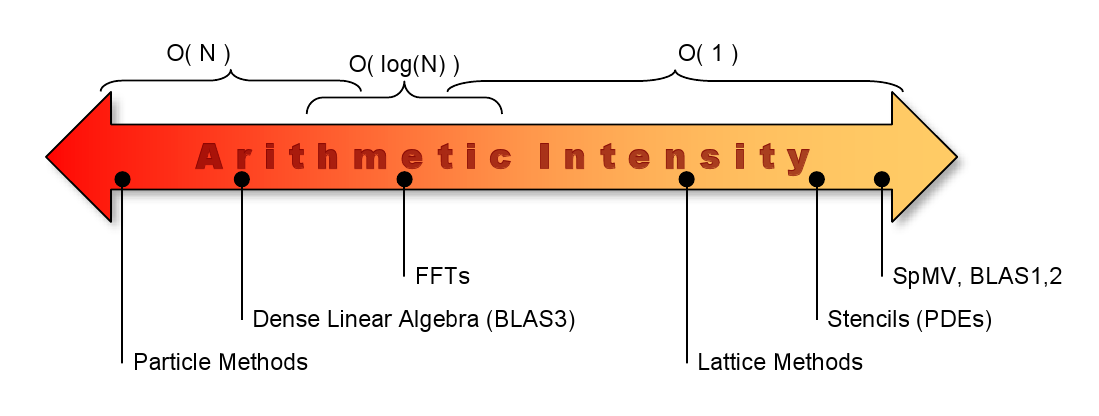
\includegraphics[width=0.85\textwidth]{figures/OlikerArithmeticIntensity} \\
    \vspace{-1em}
    {\tiny (Oliker et al. 2008)}
  \end{block}
\end{frame}
